\documentclass[utf8,14pt,a4paper,oneside,russian]{book}
\usepackage[14pt]{extsizes}
\usepackage{longtable}
\usepackage{listings}
\usepackage{mathtools}

%===========
%=Кодировка=
%===========
\usepackage[T2A]{fontenc}
\usepackage[utf8]{inputenc}
\usepackage[main=russian, english]{babel}

%===================
%=Разметка страницы=
%===================
\usepackage[left=3cm, right=1cm, top=2cm, bottom=2cm, headheight=14pt, headsep=1cm, footskip=1cm]{geometry}
\pagestyle{plain}
\linespread{1.1} %Межстрочный интервад
\setlength{\parindent}{1.25cm} %Абзацный отступ
\setlength{\parskip}{0em} %Интервал между абзацами
\usepackage{indentfirst}

\usepackage{misccorr}
\usepackage{graphicx}
\usepackage{amsmath, amssymb, amsfonts}

%===========
%=Заголовки=
%===========
\usepackage{titlesec}

\titleformat{\section}{\centering\large\bfseries}{\thesection.}{0.5em}{\MakeUppercase}
\renewcommand{\thesection}{\arabic{section}}
\renewcommand{\sectionmark}[1]{\markright{\thesection.~#1}}
\titlespacing*{\section}{0em}{2em}{1em}

\titleformat{\subsection}{\centering\normalsize\bfseries}{\thesubsection.}{0.5em}{}
\renewcommand{\thesubsection}{\arabic{section}.\arabic{subsection}}
\titlespacing*{\subsection}{0em}{1.25em}{0.5em}

\titlespacing*{\paragraph}{0em}{1.05em}{0.25em}

%============
%=Содержание=
%============
\usepackage{titletoc}
\makeatletter
\renewcommand{\tableofcontents}{\section*{Содержание}\markboth{Содержание}{}\@starttoc{toc}\newpage}
\makeatother
\titlecontents{section}[1.5em]{}{\contentslabel[\thecontentslabel.]{1.5em}}{}{\rule{0.1cm}{0pt}\titlerule*[0.75pc]{.}\contentspage}
\titlecontents{subsection}[4em]{\vspace{0.05em}}{\contentslabel[\thecontentslabel.]{2em}}{}{\rule{0.1cm}{0pt}\titlerule*[0.75pc]{.}\contentspage}

%========
%=Списки=
%========
\usepackage{enumitem}
\makeatletter
\AddEnumerateCounter{\asbuk}{\@asbuk}{м)}
\makeatother
\setlist{nolistsep, topsep=0.375em}
\setenumerate{leftmargin=2cm, labelsep=0em, labelwidth=0.75cm, align=left}
\setitemize{leftmargin=2cm, labelsep=0em, labelwidth=0.75cm, align=left}
\renewcommand{\labelitemi}{--}
\renewcommand{\labelenumi}{\arabic{enumi})}
\renewcommand{\labelenumii}{\asbuk{enumii})}
\renewcommand{\labelenumiii}{--}

%==========================
%=Математические операторы=
%==========================
\DeclareMathOperator{\mob}{Mob}
\DeclareMathOperator{\fix}{Fix}
\DeclareMathOperator{\ord}{ord}

\graphicspath{{pictures/}}
\DeclareGraphicsExtensions{.pdf,.png,.jpg}

\begin{document}

\thispagestyle{empty}
\small
\begin{center}
    
\includegraphics[width=4.55cm]{logo_mirea}\\
    \MakeUppercase{Минобрнауки России}\\[1em]
    Федеральное государственное бюджетное образовательное учреждение\\
    высшего образования\\[0.5em]
    \textbf{<<МИРЭА -- Российский технологический университет>>}\\
    \textbf{РТУ МИРЭА}\\
    \rule{\textwidth}{0.75pt}\\
    Институт Искусственного Интеллекта\\
    Базовая кафедра БК252 - информационной безопасности.\\
    
    \rule{\textwidth}{0.75pt}\\[5em]
    \normalsize\MakeUppercase{\textbf{Курсовая работа}}\small\\[0.5em]
    По дисциплине <<Криптографические методы защиты информации>>\\[0.5em]
    по теме: <<Безопасность ключевого хеширования, основанного на открытых перестановках.>>\\[1.5em]
    \begin{tabular}{p{7cm}p{6cm}c}                    \\[-0.5em]
      &                & \\[1em]
        Студент группы ККСО-03-19 & Воеводин К.А.  & \rule{2cm}{0pt}                    \\[-0.5em]
                                  &                & \\[2em]
        Преподаватель             & Бондакова О.С.  & \rule{2cm}{0pt}                    \\[-0.5em]
                                  &                & \\[5em]
    \end{tabular}
    \vfill
    Москва -- 2023
\end{center}
\normalsize
\newpage

% Содержание
\tableofcontents

% Первая глава
\newpage
\section{Введение}
Криптографические функции с двойным расширением (deck) обобщают концепцию 
кодов аутентификации сообщений (MAC) и потоковых шифров. Они поддерживают 
строки переменной длины в качестве входных данных и возвращают строки 
переменной длины в качестве выходных данных. Ярким примером строительных 
функций deck является Farfalle, который состоит из набора общедоступных 
перестановок и функций прокатки, которые используются в его слоях сжатия 
и расширения. Обобщая слой сжатия Farfalle, доказывается его универсальность 
с точки зрения вероятности различий по сравнению с используемой в нем общедоступной 
перестановкой. Поскольку уровень сжатия Farfalle по своей сути параллелен, 
он сравним с обобщением функции последовательного сжатия, вдохновленной 
Pelican-MAC. Одна и та же общедоступная перестановка может привести к 
различным универсалиям в зависимости от того, выполняется ли сжатие 
параллельно или последовательно. Параллельная конструкция неизменно работает 
лучше, чем последовательная, иногда в разы. Этот эффект возможно продемонстрировать с 
использованием Xoodoo, который представляет собой уменьшенный в округленном виде 
вариант общедоступной перестановки, используемой в deck функции Xoofff.

Ключевые слова: хэширование с ключом, общедоступные перестановки, 
универсальное хэширование, параллельное, последовательное, дифференциальная 
вероятность.



\newpage
\section{Вступление}

%\subsection{Цель}

Функция двойного расширения с криптографическим ключом \\
(deck) - относительно недавний криптографический примитив, представленный 
Daemen. Функция deck обобщает функцию MAC и потоковый шифр в том смысле, 
что она поддерживает строки переменной длины в качестве входных данных и 
возвращает строки переменной длины в качестве выходных данных.

Farfalle - это конструкция для построения функций deck из набора 
b-разрядных общедоступных перестановок и скользящих функций, 
которая была представлена в 2017 году Bertoni. Он состоит из фазы сжатия, 
за которой следует фаза расширения. Фаза сжатия состоит из двух этапов, 
а именно, генерации последовательности b-битных секретных масок переменной 
длины, за которой следует параллельное сжатие строк. Каждая b-разрядная 
секретная маска добавляется к b-разрядному блоку входной строки с помощью 
группового добавления. Затем к каждому блоку результирующей строки применяется 
общедоступная перестановка. Выходные данные всех вызовов перестановки 
суммируются, в результате чего получается переменная, называемая аккумулятором.
Farfalle - это тип функции, называемый protected hash (также называемый 
hash-then-encrypt). Целью такой функции является достижение безопасности 
псевдослучайной функции (PRF). Это определяется с точки зрения преимущества 
оптимального злоумышленника в том, что он отличает его от случайного оракула, 
когда вводится равномерно случайный ключ, неизвестный злоумышленнику. 
Защищенные хэш-функции можно описать следующим образом. 
Для функции сжатия с ключом \(F_k\) и криптографической функции \(P_k'\) 
с фиксированной длиной входного сигнала выходной сигнал Z для заданного 
входного сигнала m определяется как Z =\(P_k'\)(\(F_k\)(m)).
Теперь мы можем выделить вклад функции сжатия \(F_k\) в PRF-безопасность 
защищенной хэш-функции, предположив, что \(P_k'\) является PRP-безопасным. 
Тогда преимущество PRF защищенной хэш-функции является верхней границей 
суммы преимущества PRF и вероятности успеха, взятой по ключевому 
пространству k оптимального злоумышленника для генерации коллизий в 
выходных данных Fk: distinct m, m' таких, что \(F_k(m) = F_k(m')\).
Эта вероятность, в свою очередь, является верхней границей так называемой\\
е-универсальности F. Это максимум, принятый для всех различных пар сообщений, 
из вероятности, принятой для всех ключей k, что два различных сообщения 
приведут к одному и тому же результату. Типичным применением защищенных 
хэш-функций является вычисление кода аутентификации сообщения (MAC).


\newpage
\section{Предварительные замечания}

В этом разделе определены основные обозначения и определения, необходимые 
для проведения анализа, представленного в данной работе.

\subsection{Обозначения.}

Представленные хэш-функции работают со строками элементов абелевой 
группы ⟨G,+⟩ с нейтральным элементом, записанным как 0. 
Элементы G обозначим блоками, а набор строк l-блока как \(G^l\), 
а набор строк длиной от 1 до k как \(BS(G, k)= u^k_{l=1}  G^l\). 
В данной работе подразумевается работа с переменными \(x \in G\), 
которые имеют значение, зависящее от ключа k. 
Вероятность того, что переменная x имеет значение X, через Pr(x = X). 
Другими словами, Pr(x = X) - это доля пространства ключей, для которой 
переменная x имеет значение X. Мы называем две переменные независимыми, 
если $Pr(x = X, x' = X') = Pr(x = X) Pr(x' = X')$ для всех $X, X' \in G$.

Массовая функция вероятности (PMF) переменной x, обозначаемая как $g_x$, 
представляет собой массив значений Pr(x = X) по всем значениям X. Мы имеем 
$g_x(X)$ = Pr(x = X), причем вероятность берется по ключевому пространству. 
Очевидно, что $\forall X:0 \le g_x(X) \le 1$ и $\sum_X g_x(X)=1$. Таким образом, 
PMF можно рассматривать как отображение g: G → [0,1].

Свертка двух PMF $g_x,g_y$, обозначаемая как $g_x * g_y$, задается следующим 
образом: 

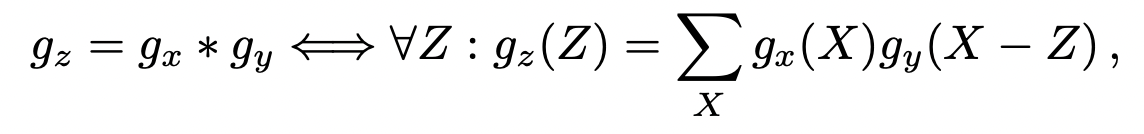
\includegraphics[width=11cm]{form1}

определяется групповой операцией G и выполненным суммированием над R.

Обозначим равномерный PMF над G через U: так, что \\
$\forall X \in G$ $U(X) = \frac {1}{\#G}$. Когда есть две 
независимые переменные x, y $\in$ G 
тогда PMF их суммы (в G) является сверткой их PMF. Более того, если z = x + y, 
причем x и y независимы, то $max_Z g_z(Z) \le min(max_X g_x(X),max_Y g_y(Y))$. 
Из этого следует, что свертка с независимой однородной переменной 
приводит к однородной переменной.

\subsection{$\varepsilon$-универсальность и $\varepsilon-\Delta$Универсальность.}

Безопасность хэш-функций с ключом в их соответствующих вариантах 
использования определяется их $\varepsilon$-универсальностью и 
$\varepsilon-\Delta$Универсальностью.

\textbf{Определение 1.} ($\varepsilon$-универсальность). Хэш-функция с ключом F 
называется $\varepsilon$-универсальной, если для любых 
различных строк m, $m^*$:

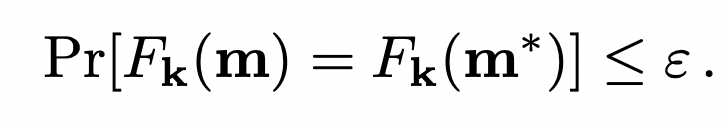
\includegraphics[width=8cm]{form2}

\textbf{Определение 2.} ($\varepsilon-\Delta$Универсальность). Хэш-функция с ключом F 
называется $\varepsilon-\Delta$Универсальной, если для любых различных 
строк m, $m^*$ и для всех $\Delta \in$ G:

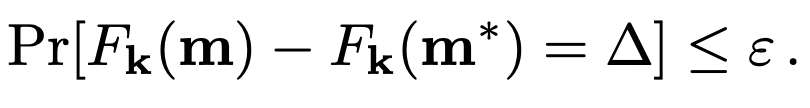
\includegraphics[width=8.5cm]{form3}

\subsection{Функции 'Ключ-затем-хэш/Key-Then-Hash'}

Мы изучаем хэш-функции с ключами, которые принимают в качестве входных 
элементов BS(G, k) и возвращают элемент G. Ключи являются элементами $G^k$. 
При обработке входных данных сначала к входным данным добавляется ключ, 
а затем к результату применяется функция без ключа. Мы называем этот 
частный случай хэш-функций с ключом "ключ-затем-хэш-функции". Функция 
"ключ-затем-хэш" обозначается как F и определяется как $F: G^k * $BS(G, k) → G 
с $F_k(m) = F (k + m)$. Сложение двух строк m, $m^*$ с $|m| \le |m^*|$ определяется 
как m' = m+$m^*$ = $m_1$ +$m^*_1$,$m_2$ + $m^*_2$,...,$m_{|m|}$ +$m^*_{|m|}$, таким образом, сумма 
двух строк такой же длины, как самый короткий из двух.

\subsection{Дифференциальная вероятность для функций фиксированной длины.}

\textbf{Определение 3.}(Дифференциальная вероятность). Дифференциальная вероятность 
дифференциала (a, b) над перестановкой f : G → G, 
обозначаемая как DPf (a, b), равна:

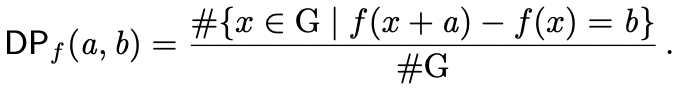
\includegraphics[width=9cm]{form4}

Мы говорим, что входная разность a распространяется на выходную 
разность b с вероятностью DPf (a, b). 

Если DPf (a, b) > 0, мы называем входную разность a и выходную р
азность b совместимыми через f. В наших границах $max_{a\neq0,b}$ $DP_f$(a,b) 
играет важную роль, и мы обозначаем это через $MDP_f$ . Дифференциальные 
вероятности всех дифференциалов с общей входной разностью a образуют PMF, 
который мы обозначаем как $DP_a$, таким образом, мы имеем $DP_a$(b) = $DP_f$(a,b).

\newpage
Полезной величиной является Евклидова норма $DP_a$, \\
заданная через $\sum_b DP^2_a(b)$. Мы обозначим это через $NDP_f(a)$ и обозначим максимум этой нормы по всем 
входным разностям через $MNDP_f$, следовательно, $MNDP_f= max_{a\neq0} \sum_b DP^2_f (a, b)$.

\subsection{Различия между хэш-функциями "Ключ-затем" и их дифференциальная вероятность.}

Классически определение дифференциала определяется над функциями фиксированной 
длины. Введение входных данных переменной длины делает определение 
дифференциала нетривиальным из-за того факта, что две строки могут 
отличаться не только по значению, но и по длине. В этом разделе мы 
обобщаем концепцию дифференциалов на функции переменной длины и 
определяем дифференциальную вероятность таких дифференциалов по сравнению 
с функциями key-then-hash. Суть наших доказательств в разделах 
основана на понимании взаимосвязи между вероятностью дифференциалов ключевой 
хэш-функции и вероятностями лежащей в ее основе перестановки.

\textbf{Предложение 1.} Для хэш-функции "ключ-затем" вероятность того, что два 
сообщения m, $m^*$ с $|m| \le |m'|$ приведут к разнице выходных данных 
$\Delta$ через $F_k$, определяется следующим соотношением:

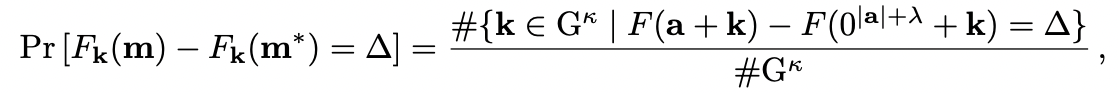
\includegraphics[width=15cm]{form5}

где $\lambda=|m'|-|m|$ и a взята как $a\in G^{|m|}$, такая что $t_m=a+m^*$.

\textbf{Определение 4.} (разница между двумя строками). Мы определяем разницу между
двумя строками $m,m^*$ с $|m| \le |m^*|$ как пару (a,$\lambda$) $\in G|m| ×Z \ge 0$, где 
$a = m_1 - m^*_1, m_2 - m^*_2,...,m_{|m|} - m^*_{|m|}$ и $\lambda =|m^*| - |m|$.

Когда $\lambda$ = 0, мы говорим, что разница равна длине, а в противном 
случае мы говорим, что она неодинаковой длины. Теперь мы определяем 
вероятность различий по F.

\textbf{Определение 5.} (Обобщенные дифференциалы и их DP). Учитывая \\
входную разность (a, $\lambda$) и выходную разность $\Delta$, дифференциальная вероятность 
дифференциала (a, $\lambda, \Delta$) по F, обозначаемая как $DP_F$ (a, $\lambda, \Delta$),
 определяется как:

 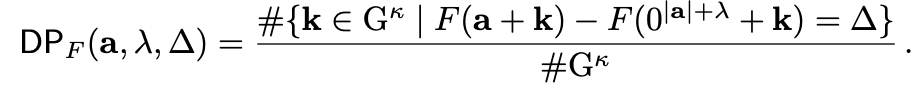
\includegraphics[width=13.5cm]{form7}

 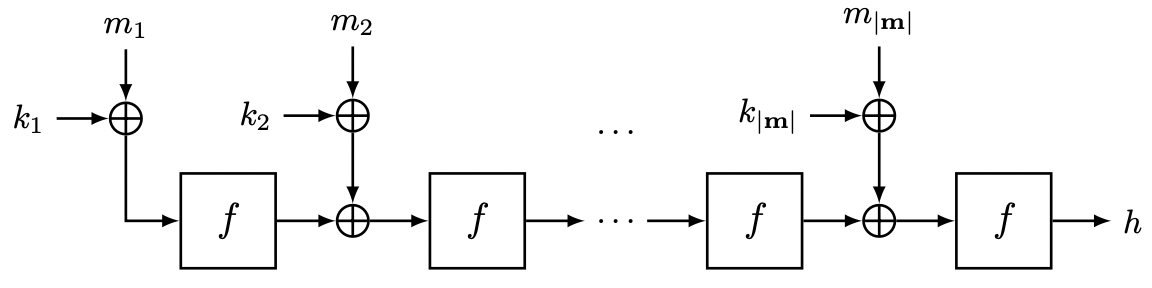
\includegraphics[width=13.5cm]{form8}

\begin{center}
  Рисунок 1: Серийный номер сериализации[f].
\end{center}

Чтобы упростить обозначения, когда $\lambda = 0$, опустим его из \\
дифференциала. Если мы примем $\lambda$ = 0 и a = a $\in$ G, то получим 
классическое определение дифференциальной вероятности.
Что касается функций фиксированной длины, то дифференциальные 
вероятности всех дифференциалов с общей входной разностью (a,$\lambda$) 
образуют PMF, который мы обозначаем как $DP_F(a,\lambda)$, поэтому мы 
имеем $DPF (a,\lambda)(\Delta) = DPF (a, \lambda, \Delta)$. 
Из определений 1 и 2 мы можем сказать, что ключевая хэш-функция F 
является $max_a, \lambda DP_F (a, \lambda, 0)$ -универсальной и 
$max_{a, \lambda, \Delta} DP_F (a, \lambda, \Delta)$ -$\Delta$универсальной. 
В остальной части статьи будет акцент на доказательстве верхних границ 
дифференциальной вероятности конструкций.

\section{Построение последовательного ключа с последующим хэшем.}

Рассмотрим универсальность последовательных функций "ключ-затем-хэш", 
основанных на неконтролируемой перестановке f. Конструкция описана в 
разделе 4.1. Основная теорема приведена в разделе 4.2. Универсальность 
такой конструкции равна максимальной дифференциальной вероятности по 
всем нетривиальным дифференциалам лежащей в основе перестановки. 
Докажем теорему 1 в разделе 4.3.

\subsection{Конструкция.}

Определение сериализации общедоступной перестановки в алгоритме 1. 
Конструкция принимает в качестве параметров общедоступную 
перестановку f : G → G и максимальную длину строки k. 
Его входными данными являются ключ k $\in G^k$ и сообщение m $\in$ BS(G, k), 
и он возвращает дайджест h $\in$ G.

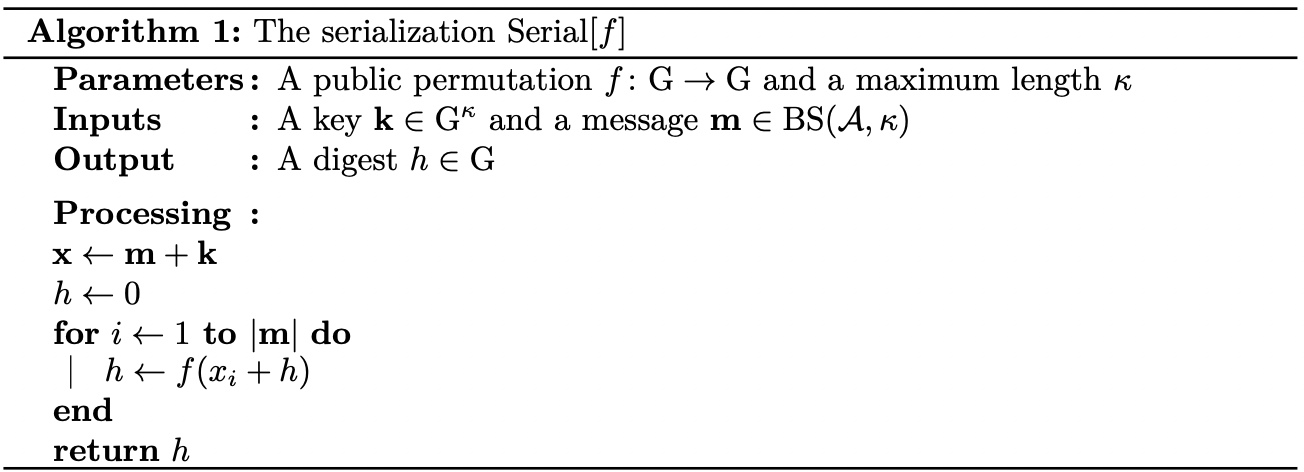
\includegraphics[width=14cm]{form9}

\subsection{Безопасность серийной конструкции.}

Универсальность сериализации общедоступной перестановки f в терминах 
вероятности дифференциалов по f. Докажем, что последовательный [f] равен
$\varepsilon$-универсальный и $\varepsilon$-$\Delta$универсальный для 
одного и того же значения $\varepsilon$.

\textbf{Теорема 1.} (Универсальность последовательного[f]). Сериализация 
общедоступной перестановки f, Serial[f], является $MDP_f$-универсальной и \\
$MDP_f$ - $\Delta$универсальной.

\subsection{Доказательство теоремы 1.} 

Для того, чтобы определить вероятность различий по последовательному
[f](a,$\lambda, \Delta$), обозначаемому как DPS, следует учитывать 
различия как в равной, так и в неодинаковой длине. В лемме 1 показано, 
что все дифференциалы с входными разностями неодинаковой длины имеют \\
$DP_S = \frac {1}{\#G}$ независимо от a и $\Delta$. В лемме 2 доказываются 
рекурсивное выражение для $DP_S$ для разностей равной длины при |a| > 1. 
Объединив эти две леммы, возсожно доказать теорему 1.

\textbf{Лемма 1.} (DPS с разностями неодинаковой длины). Для любого \\
дифференциала (a, $\lambda, \Delta$) с $\lambda$ > 0, $DP_S = \frac {1}{\#G}$.

\textbf{Доказательство.} Пусть m,$m^*$ - две строки с длиной |m| < |$m^*$| и 
разностью (a, $\lambda, \Delta$). Вероятность того, что 
последовательный[f](m + k) = x равен $\frac {1}{\#G}$, поскольку он является 
результатом $f(cv + k_{|m|} + m{|m^*|})$,, где cv - промежуточное значение, 
накапливающее первые блоки |m| - 1. Поскольку мы берем вероятность по всем 
ключам и, следовательно, по всем значениям $k_{|m|}$, распределение вероятностей
входных данных перестановки является равномерным, а следовательно, и ее 
выходных данных. Аналогично, вероятность того, что 
последовательный $[f](m^* +k) = y$ равен $\frac {1}{\#G}$, 
поскольку он является результатом $f(cv^* +k_{|m^*|} +m_{|m^*|})$, 
где $cv^*$ - промежуточное значение, накапливающее первые блоки $|m^*|$ - 1. 
Значение y не зависит от значения x, поскольку они являются результатом 
вычисления f при сложении $k_{|m|}$ и $k_{|m^*|}$
соответственно, они представляют собой два блока секретных ключей, выбранных 
независимо друг от друга из равномерного распределения. Мы получаем, что 
выходная разница равна $\Delta$, если x = $\Delta$ + y. Следовательно, мы
можем разделить пространство выборки. Мы используем следующее условие. 
Последовательный $[f](m + k) = \Delta + y$ при заданном событии 
последовательность $[f](m^* + k) = y$. Каждое разбиение имеет 
вероятность $\frac {1}{\#G^2}$ . Применяя по закону полной вероятности 
мы получаем выражение из леммы 1.

\textbf{Лемма 2.} ($DP_S$ дополнительного блока сообщений с $\lambda$ = 0).
Пусть (a, a) - объединение a $\in$ BS(G, k) и a $\in$ G. Дифференциальная 
вероятность дифференциала ((a, a), $\Delta$) по последовательности[f] 
задается формулой:

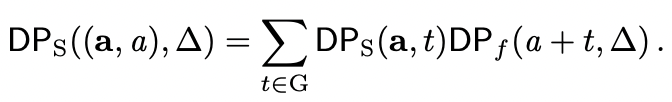
\includegraphics[width=10cm]{form10}

\textbf{Доказательство.} Докажем это, используя закон полной вероятности. 
Рассмотрим условную вероятность того, что a + t распространяется на $\Delta$ 
через f, учитывая, что a распространяется на t через последовательность [f] 
для любого значения t $\in$ G. Поскольку ключевые блоки выбираются независимо 
и случайным образом из равномерного распределения, эти два события независимы 
друг от друга. Следовательно, это происходит с вероятностью 
$DP_S(a, t)DP_f (a + t, \Delta)$. Применяя закон полной вероятности, получаем 
выражение из леммы 2.

\textbf{Теорема 1.} Используя лемму 2, докажем, что DP дифференциала 
равной длины ((a, a), $\Delta$) сверху ограничен 
$max_{\Delta'} DP_S$(a, $\Delta'$):

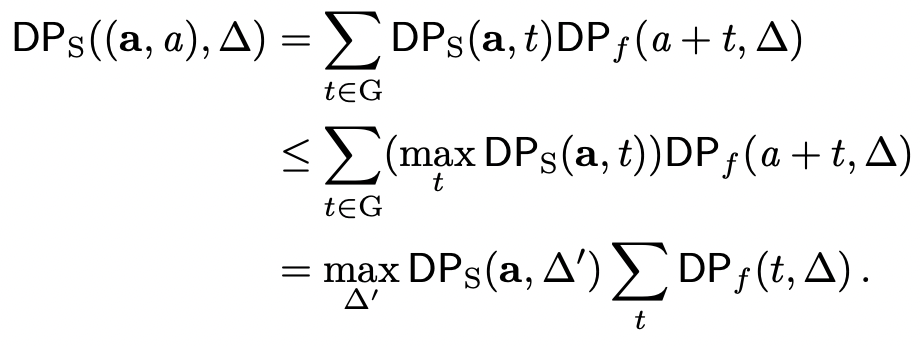
\includegraphics[width=11cm]{form11}

Поскольку f - это перестановка, мы имеем: \\
$\sum_t DP_f(t,\Delta) = \sum_t DP_{f^-1}(\Delta, t) = 1$ и мы получаем:

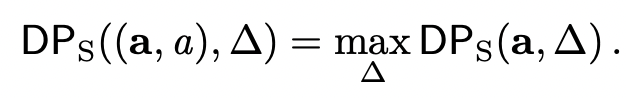
\includegraphics[width=8.5cm]{form12}

Поскольку (1) справедливо для любой входной разности (a, a) и
 выходной разности $\Delta$, мы имеем: 

 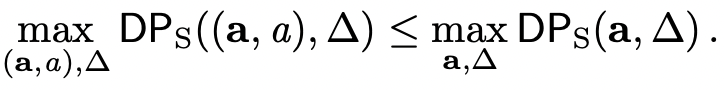
\includegraphics[width=8.5cm]{form13}

 Отсюда следует, что максимальный DP для всех дифференциалов равной длины 
 с входной разностью длины l ограничен сверху максимальным DP для всех 
 дифференциалов равной длины с входной разностью длины l - 1. Это можно 
 применять рекурсивно, пока мы не достигнем l = 1, что дает 
 $max_{a_1},\Delta DP_S(a_1, \Delta) = max_{a_1},\Delta DP_f (a_1, \Delta) = MDP_f$ . 
 Таким образом, максимальный DP для всех дифференциалов равной длины 
 равен $MDP_f$ .

 Для дифференциалов неодинаковой длины лемма $\frac {1}{\#G}$ утверждает, 
 что DP равен 1 . Как $MDP_f > \frac {1}{\#G}$, на этом доказательство заканчивается.
 
 \section{Параллельное построение ключ-затем-хэш конструкции}

Рассмотрим универсальность конструкции, основанной на неконтролируемой 
перестановке f. Однако в этой конструкции строки сжимаются параллельным 
образом. В разделе 5.1 определена конструкцию. Основные теоремы этого 
раздела приведены в разделе 5.2. В разделах 5.3 и 5.4 доказательство 
теоремы 2 и 3 соответственно.

\subsection{Конструкция.}

Описание распараллеливания общедоступной перестановки в алгоритме 2 
и изображение на рисунке 2. Конструкция принимает в качестве параметров 
общедоступную перестановку f : G → G и максимальную длину строки k. 
Входными данными являются ключ k $\in G^k$ и строка m $\in$ BS(G, k), 
и она возвращает дайджест h $\in$ G.

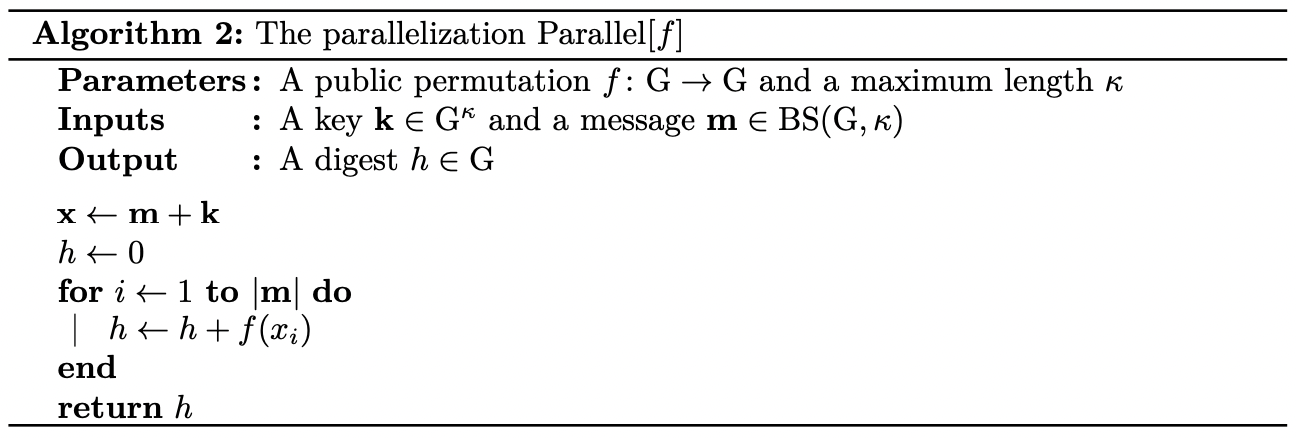
\includegraphics[width=15cm]{form14}

\subsection{Безопасность параллельного построения.}

В этом разделе мы опишем универсальность распараллеливания открытой 
перестановки f в терминах дифференциальной вероятности f. В отличие от 
сериализации общедоступной функции, $\varepsilon$-универсальность и 
$\varepsilon-\Delta $ универсальность Parallel[f] в целом различны.

\textbf{Теорема 2.} ($\Delta$-универсальность параллели[f]). Распараллеливание \\
публичной перестановки f, Parallel [f], является $MDP_f-\Delta$универсальным.

\textbf{Теорема 3.} (Универсальность параллели[f]). Распараллеливание 
публичной перестановки f, Parallel [f], является $MNDP_f$-универсальным.

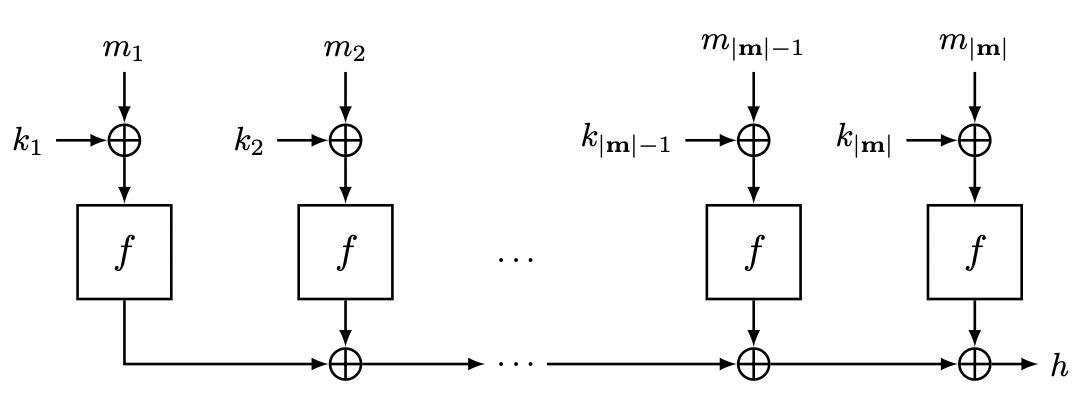
\includegraphics[width=15cm]{form15}
\begin{center}
  Рисунок 2: Параллельное распараллеливание[f].
\end{center}

\subsection{Доказательство теоремы 2.}

В лемме 3 показано, что PMF входной разности для параллели[f], 
обозначаемый как $DP_{P(a,\lambda)}$, может быть получен путем свертки 
$PMF_S DP_{a_i}$ и равномерного распределения U.

\textbf{Лемма 3.} (DP дифференциалы над параллелью[f]). PMF входной разности 
(a$\lambda$) для параллели[f] задается формулой:

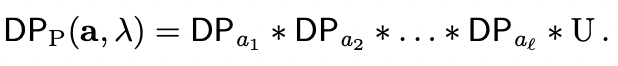
\includegraphics[width=9cm]{form16}

\textbf{Доказательство.} Предположим, мы обрабатываем слева направо. 
Выразим PMF значения цепочки после обработки нового блока с разницей a как 
функцию PMF значения цепочки перед обработкой этого нового блока. Обозначаем 
разницу в частичном сообщении через a. Согласно определению, которое имеем 
для PMF этого значения цепочки $DP_{P(a)}$. PMF разницы в новом блоке равен 
$DP_a$. Новое значение значения цепочки является суммой этих двух переменных. 
Если PMF независимы, то результирующий PMF задается сверткой этих двух. 
Эти PMF действительно независимы, поскольку два PMF управляются 
неперекрывающимися блоками ключей и их распределение осуществляется по 
всем возможным ключам. Это может быть применено рекурсивно, и мы получаем 
для любых двух частичных сообщений равной длины, что 
$DP_{P(a)} = DP_{a_1} DP_{a_2} . . . DP_{a_{|a|}}$ .

Теперь рассмотрим новый блок, который присутствует только в одном из двух 
сообщений. Разница между двумя сообщениями теперь заключается просто в 
значении выходных данных перестановки для блока ввода в самом длинном 
сообщении. PMF этого значения представляет собой распределение U в качестве 
входных данных из-за наличия ключевого блока. Новое значение значения цепочки 
является суммой этих двух переменных. Эти PMF независимы, поскольку два PMF 
здесь также управляются неперекрывающимися блоками ключей. Следовательно, 
PMF суммы является сверткой PMF. Свертка с равномерным распределением 
снова дает равномерное распределение.

Объединение двух результатов доказывает лемму.

\textbf{Теорема 2.} Аналогично доказательству теоремы 1, докажем верхнюю 
границу $max_{a,\lambda,\Delta} DP_P(a, \lambda, \Delta)$.

Применяя лемму 3, получаем следующие верхние границы:

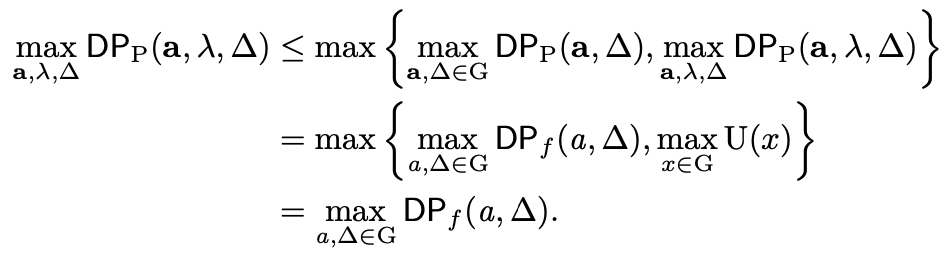
\includegraphics[width=13cm]{form17}

\subsection{Доказательство Теоремы 3.}

В этом разделе доказательство теоремы 3, использующее тот же метод, 
который использовался при доказательстве теоремы 2, но на двухблочных 
дифференциалах равной длины.

\textbf{Теорема 3.} Поскольку f - это перестановка, невозможно достичь 
разности выходных данных 0 при разнице в длине одного блока. Из 
доказательства теоремы 2 мы знаем, что справедливо следующее:

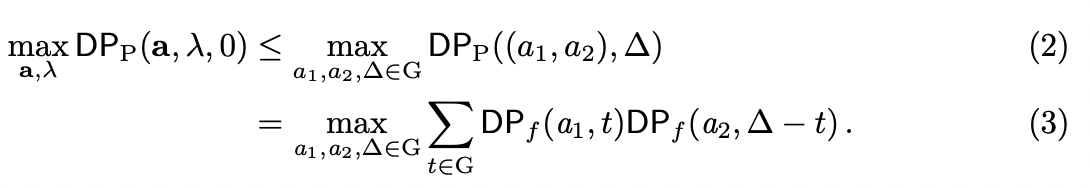
\includegraphics[width=15cm]{form18}

Правую часть (3) можно рассматривать как скалярное произведение 
векторов с компонентами, проиндексированными через t. Скалярное 
произведение двух векторов является верхней границей максимума 
нормы двух векторов, где нормой вектора является сумма квадратов 
его координат. Следовательно, имеем следующую верхнюю границу:

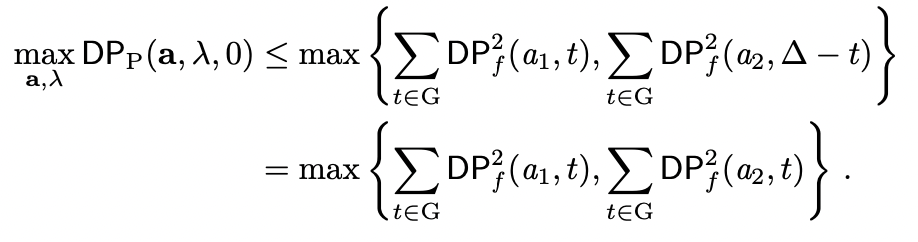
\includegraphics[width=13cm]{form19}

Это верно для любого $a_1$ или $a_2$, следовательно, имеем:

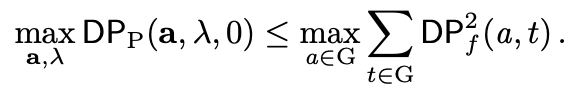
\includegraphics[width=8cm]{form20}

Равенство достигается путем принятия $a_2 = -a_1$.

\section{Приложение к Xoodoo.}

В этом разделе определяем, привязываем и оцениваем количества Xoodoo,\\ 
которые определяют универсальности в ключевых хэш-конструкциях: 
$MDP_f$ и $MNDP_f$ . В разделах 6.1 и 6.2 предоставлены некоторые базовые 
знания, необходимые для понимания этого раздела. В разделах 6.3 и 6.4 
обсуждаются $MDP_f$ и $MNDP_f$ Xoodoo[3] и Xoodoo[4] соответственно.

Из теоремы 1 непосредственно вытекает MDPf -универсальность и\\
$MDP_f$ -$\Delta$универсальность последовательных [Xoodoo[3]] и последовательных 
[Xoodoo[4]], а из теорем 2 и 3 вытекает $MDP_f$ -$\Delta$универсальность и 
MNDPf -универсальность параллельных [Xoodoo[3]] и параллельных [Xoodoo[4]].

\subsection{Основа дифференциального распространения.}

Поскольку рассматриваются только дифференциальные вероятности по f, 
просто напишем DP для $DP_f$. Определение DP дифференциалов по повторяющейся 
перестановке проходит через дифференциальные трассы: цепочку дифференциалов 
по последовательности последовательных раундов.

\textbf{Определение 6.} (Дифференциальный след). r-образный дифференциальный 
след, обозначаемый как Q, представляет собой последовательность из r + 1 
разностей: входной разности, r - 1 промежуточных разностей и выходной 
разности, где круглые разности $(q_{i-1},q_i)$ имеют ненулевое 
значение DP, а именно:

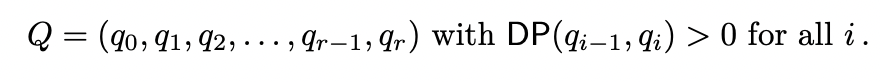
\includegraphics[width=13cm]{form21}

Дифференциальная вероятность следа, обозначаемая DP(Q), представляет 
собой вероятность того, что случайная пара с входной разностью $q_0$ 
распространяется через промежуточные разности $q_1, q_2$, ... до выходной 
разности $q_r$.

Полезной концепцией при изучении дифференциального распространения 
является вес ограничения. 

\textbf{Определение 7.} (Ограничительный вес дифференциала [9]). 
Ограничительный вес дифференциала DP(a, b) > 0 определяется как 
$w(a, b) = - log_2 DP(a, b)$.

\textbf{Определение 8.} (Ограничительный вес дифференциального следа [9]). 
Вес ограничения дифференциального следа $Q = (q_0, q_1, . . . , q_{r-1})$ 
определяется как $w(Q) = \sum_i w(q_{i-1}, q_i)$, следовательно, 
сумма весов ограничения, если его дифференциалы округлены.


В дальнейшем будет опущено уточнение “ограничение” и уточнения пойдут 
только о весе. Используется термин "весовой профиль трассы" для обозначения 
последовательности весов ее круглых дифференциалов. Вес любого заданного 
дифференциала по кругу, как правило, легко вычислить, а следовательно, и 
вес любого заданного следа. Часто $2^{-w (Q)}$ является хорошим приближением для 
DP (Q). Если распространение через круглые дифференциалы следа независимо, 
мы называем его марковским следом, и он удовлетворяет DP (Q) = $2^{-w (Q)}$. 
В целом это не так, и это момент внимания, который необходимо проверить. 
Трассы связаны с дифференциалами: DP дифференциала r-round - это сумма $DP_S$ 
всех трасс, соединяющих входную разность и выходную разность:

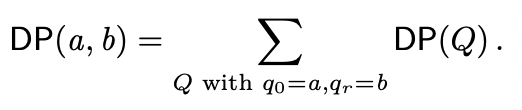
\includegraphics[width=7cm]{form22}

Пути с общей разницей входных и выходных данных вносят вклад в одну и ту же 
разницу и, как говорят, группируются. Мы называем тропу, которая является 
единственной в своем роде, одинокой тропой.

В статьях, посвященных поиску троп, часто сообщается о больших наборах 
троп с общими особенностями, а не об отдельных тропах. Эти наборы называются 
ядрами трассировки.

\textbf{Определение 9.} (Ядро дифференциального следа [17]). Ядро 
дифференциальной трассы r-раунда, обозначаемое как Q, представляет собой 
набор дифференциальных трасс по r раундам с общим ядром промежуточных 
различий: $(q_1, q_2, ..., q_{r-1})$ с DP$(q_i, q_{i+1}) > 0$ для всех 1 $\le i < r - 1$.

Учитывая r-образное ядро трассировки Q и r-образный дифференциал (a, b), 
ядро трассировки будет вносить вклад в DP (a, b), если a совместимо с 
$q_1, q_{r-1}$ с b.
Определение $NDP_f(a)$ требует вычисления DP(a, b) для всех выходных 
разностей b, а в типичных повторяющихся перестановках это неосуществимо. 
Однако разумно предположить, что для заданной входной разности a известны 
все выходные разности b с DP(a, b) > T. Тогда мы можем использовать 
следующую лемму для определения верхней границы $NDF_f(a)$.

\textbf{Лемма 4.} Для любого предела T мы имеем:

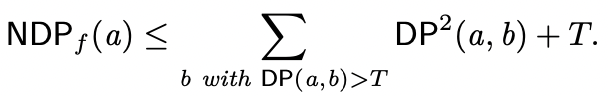
\includegraphics[width=8cm]{form23}

\textbf{Доказательство.} Разбиение дифференциалов на части дает:

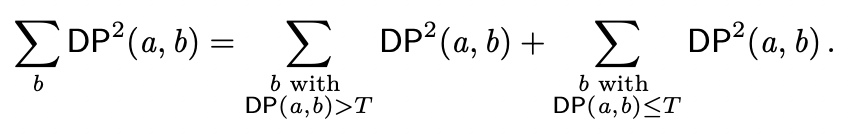
\includegraphics[width=10.5cm]{form24}

Вторая сумма в правой части равна не более T, а именно, используя 

$\sum_b DP(a, b) = 1$ даёт:

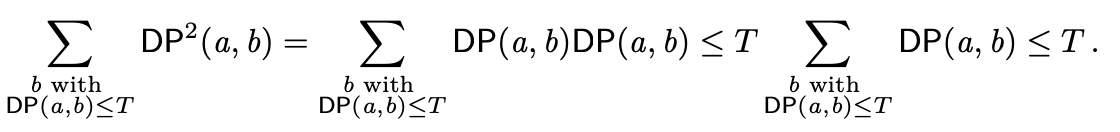
\includegraphics[width=13.5cm]{form25}

Это доказывает лемму.

\subsection{Дифференциальное распространение в Xoodoo.}

Xoodoo - это семейство 384-битных перестановок с классической итеративной 
структурой: оно итеративно применяет функцию округления к состоянию. 
Он параметризуется количеством раундов: Xoodoo с r раундами обозначается 
Xoodoo[r]. Круглая функция состоит из линейного слоя, который мы будем 
называть $\lambda$, за которым следует нелинейный слой, называемый x. 
Нелинейный слой имеет алгебраическую степень два. Следствием этого 
является то, что в круглых дифференциалах значение DP(a,b) полностью 
определяется входной разностью a и, следовательно, одинаково для всех 
совместимых выходных разностей b[11]. Более того, обратная x также имеет 
алгебраическую степень 2, и поэтому в круглых дифференциалах значение 
DP(a, b) также полностью определяется выходной разностью b и, следовательно, 
одинаково для всех совместимых входных разностей a. Следствием этих двух 
свойств является то, что все трассы в ядре трассы имеют одинаковый вес, 
и мы можем говорить о w(Q) без двусмысленности, причем w(Q) - вес любой 
трассы в ядре.

Благодаря инвариантности к сдвигу функции Xoodoo round, маршруты 
(и ядра маршрутов) встречаются в классах с членами, которые эквивалентны 
при горизонтальных сдвигах. Эти классы имеют размер $2^d$ с d в диапазоне 
от 0 до 7. Подавляющее большинство ядер trail относятся к классам 
размером 27 = 128.

Нелинейный уровень x работает параллельно и независимо над 3-разрядными 
частями состояния, так называемыми столбцами: это слой обратимых нелинейных 
S-блоков. Это имеет свои последствия для кластеризации. Ядро следа Q вносит 
вклад в дифференциал (a, b), если a и $q_1$ совместимы. Входная разность 
a полностью определяет разность на входе x первого раунда: это $\lambda(a)$. 
Таким образом, $\lambda(a)$ и $q_1$ должны быть совместимы по x.

Ненулевая разница в столбце на входе x может распространяться только на 
ненулевую разницу на его выходе, а нулевая разница в столбце на его входе 
может распространяться только на ненулевую разницу на его выходе. Таким 
образом, $\lambda(a)$ должно быть активным точно в тех же столбцах, что 
и $q_1$. Мы говорим, что $\lambda(a)$ и $q_1$ должны иметь одинаковый 
шаблон активности столбца. Аналогично, $\lambda(q_{r-1})$ и b должны 
иметь одинаковый шаблон активности столбца.

Из этого следует, что след в ядрах следа Q может кластеризоваться 
только со следом в ядре следа Q', если $q_1$ и $q_1'$ имеют одинаковый 
шаблон активности столбца и если $q_{r-1}$ и $q'_{r-1}$ имеют одинаковый 
шаблон активности столбца.

\subsection{$MDP_f$ и $MNDP_f$ от Xoodoo.}

В репозитории Xoodoo GitHub доступен список всех 3-раундовых классов 
trail core Xoodoo с весом до 52. В списке 201 запись. Сообщается, что 
все трассы с 3 кругами и весом до 50 кг являются одиночными марковскими 
трассами. Наименьший вес 36, достигается с помощью 4-х классов 
trailcoreclasses, следовательно, по разумным предположениям, мы имеем 
$MDP_F =2^{-36}$. Предполагается, что нет ядер trail с весом выше 50, 
кластеризующихся для формирования дифференциала с DP > $2^{-36}$. 
Это потребовало бы кластеризации по меньшей мере $2^{54-36}$ = $2^18$ 
марковских трасс. Тот факт, что существует только 201 базовый класс 
trail с весом ниже 52, который содержит только одиночные марковские 
трассы, делает это крайне маловероятным.

Для оценки $MNDP_f$ интересно использовать лемму 4. Для его применения 
нам нужно сделать разумное предположение о пределе T. Если трассы остаются 
одиночными марковскими трассами до некоторого веса, например, 70, DP 
дифференциалов совпадает со значениями, предсказанными весами трасс, и мы 
можем принять T = $2^{-54}$. Очевидно, что по мере увеличения веса 
трасс вероятность кластеризации и зависимости круглых различий действительно 
возрастает. Тем не менее, маловероятно, что эти эффекты заметны для трасс 
в неприсоединенных перестановках, таких как Xoodoo, если только их вес не 
близок к ширине перестановки. Для Xoodoo это 384, что очень далеко от 50.

\newpage
\textbf{Лемма 5.} Предполагая, что все дифференциалы с DP(a, b) > T 
для T > $2^{-54}$ соответствуют одиноким марковским алгоритмам, мы 
можем определить верхнюю границу $MNDP_f$ как:

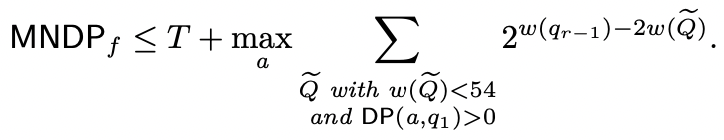
\includegraphics[width=10cm]{form26}

\textbf{Доказательство.} Вклад ядра трассировки Q в $NDP_f$ (a) отличен от нуля только 
в том случае, если $q_1$ совместим с a, и в этом случае он равен 
$2^{w(q_{r-1})-2w(Q)}$. А именно, в ядре трассировки с $q_1$, совместимым 
с заданной входной разностью a, имеется $2^{w (q_{r-1})}$ трассы, 
каждая из которых имеет DP, равный $2^{-w(Q)}$.

Чтобы два ядра trail вносили вклад в $NDP_F$ (a) при некотором значении a, 
они должны иметь одинаковые шаблоны активности столбцов в $q_1$. 
Или, другими словами, два ядра trail, которые имеют разные шаблоны 
активности столбцов в $q_1$, не могут оба вносить вклад в $NDP_F$ (a) 
для некоторого a. Мы можем разделить ядра trail на 201 класс trail core 
в соответствии с их шаблоном активности в $q_1$: мы называем эти классы 
активности. Затем для каждого разбиения мы просто добавляем вклады ядер 
трассировки, как в лемме 5.

По всем 3-раундовым ядрам трассировки, те, которые имеют наибольший вклад 
в $MNDP_f$ (a) для некоторой входной разницы, имеют вес профиля (4,4,28) 
и их вклад $2^{28-2*36} =2^{-44}$. Их три и называются одноорбитальными 
вентиляторами. Для каждого одноорбитального вентилятора есть 4 других 
следовых ядра с таким же характером активности столбца в $q_1$, которые 
вносят вклад в $MNDP_f (a)$ соответственно $2^{-54}, 2^{-54}, 2^{-56}$ и 
$2^{-58}$, что приводит к $2^{-44} + 2^{-53} + 2^{-56} + 2^{-58} + T$ = 
$(1,00226) * 2^{-44} + T$ . Все остальные классы основных классов trail 
приводят к более низким значениям для $NDP_f$ (a). Мы видим, что в 
значении $NDP_f$ (a) доминирует его “самое легкое” ядро trail и что 
дополнительные ядра trail повышают его лишь незначительно. Мы считаем 
разумным ожидать, что это также относится к (неизвестным) ядрам trail с 
весом выше 52. Тем не менее, для того, чтобы $MNDP_f$ значительно 
отклонялся от $2^{-44}$, T должно было бы увеличиться до $2^{-45}$ или 
около того, что подразумевало бы значительную кластеризацию и/или 
немарковские следы.

Таким образом, мы приходим к выводу, что $MNDP_f \approx 2-44$, и это 
значение отражает вклад одноорбитального веера в качестве доминирующего 
ядра следа. Мы видим, что для Xoodoo $MDP_f$ в 28 раз больше $MNDP_f$ .

\subsection{$MDP_f$ и $MNDP_f$ от Xoodoo. Продолжение.}

Ядра trail в Xoodoo гораздо менее документированы, чем в Xoodoo. 
Тем не менее, трассы с 4 кругами с наименьшим 
весом имеют вес 80, и документирует эти основные классы трасс, только 2 
из них.

Неизвестно, являются ли трассы в этих классах trail core марковскими 
трассами. Более того, они обладают высокой степенью симметрии, и ядра 
следов в классах группируются по два. Предполагая, что марковские следы и 
кластеризация больше не происходит, это дало бы $MDP_f = 2^{-79}$. 
Основываясь на аргументах, мы не ожидаем, что немарковское поведение 
и/или дополнительные маршруты кластеризации существенно повлияют на это 
значение.

Для $MNDP_f$ нам нужно еще раз взглянуть на весовые профили сердечников 
trail. Таковыми из двух основных классов trail являются соответственно 
(32, 24, 16, 8) и (8, 16, 24, 32).

Если мы аппроксимируем $MNDP_f$ вкладом ядер с одним следом, то первое 
даст $NDP_F (a) \approx 2^{-160 + 32} = 2^{-128}$, а второе 
$NDP_f (a) '\approx' 2^{-160 + 8} = 2^{-152}$. Однако, как уже было сказано, 
ядра trail группируются по два: кластеризующиеся ядра trail имеют равные 
различия $q_1$ и разные различия $q_3$, но с одинаковыми паттернами 
активности. При фиксации входной разности a в каждом ядре трассировки 
имеется $2^{32}$ трассы для различных выходных разностей b, все с весом 80. 
Среди этих $2^{33}$ выходных различий есть ровно $2^{16}$, куда поступают два 
маршрута, и, следовательно, они имеют DP(a, b) = $2^{-79}$. Итак, 
предполагая, что все эти трассы являются марковскими трассами, их вклад 
в $NDP_f$ (a) равен $(2^{33} - 2^{16})2^{-160} + 2^{16}2^{-158} 
= (2^{33} + 2^{163})2^{-160} = 1.00005 * 2^{-127}$.

Из-за ограниченных знаний о трассах с 4 кругами мы не можем сказать, 
нет ли ядер трасс, которые приводят к более низкому значению $MNDP_f$. 
Тем не менее, интересным наблюдением является то, что предварительное 
значение $MDP_f$ в $2^{48}$ раз выше, чем у $MNDP_f$.


\newpage
    \section{Заключение}
    
    Предполагая длинные независимые ключи, мы можем идеализировать фазу 
    сжатия Farfalle. Это предположение позволило нам изучить класс 
    хэш-функций с ключом, которые сначала добавляют ключ к входной строке, 
    а затем выполняют обработку без ключа. Мы изучаем это, сначала обобщая 
    понятие дифференциалов по указанному классу хэш-функций с ключами, также 
    принимая во внимание разницу в длине между двумя входными строками. 
    Затем мы покажем, что универсальность наших конструкций можно выразить 
    в терминах вероятности различий по лежащей в основе общедоступной 
    перестановке. В случае последовательных функций key-then-hash мы 
    показываем, что универсальность и $\Delta$универсальность задаются 
    $MDP_f$ общедоступной перестановки. Эти верхние границы являются 
    жесткими и достигаются парами сообщений одинаковой длины с разницей в 
    сообщениях длиной 1. Для параллельных функций key-then-hash мы покажем, 
    что универсальность задается $MNDP_f$ , а универсальность $\Delta$ 
    задается $MDP_f$ . Эти верхние границы снова являются жесткими и 
    достигаются парами сообщений одинаковой длины с разницей в сообщениях 
    длиной 2 и 1 соответственно. В то время как $MDP_f$ является очень 
    хорошо известным свойством публичных перестановок, $MNDP_f$ все еще 
    недостаточно хорошо изучен. Для многих общедоступных перестановок 
    $MNDP_f$ значительно меньше, чем $MDP_f$, что делает их очень 
    убедительным аргументом для использования их в параллельном режиме 
    key-then-hash вместо последовательного.

\end{document}